\def \kaflanr {12}
\lecture[\kaflanr]{\kaflanr. Tvöföld heildi}{lecture-text}
\date{11.~febrúar 2015}
\newcounter{mycount}
\refstepcounter{mycount}

\begin{document}

\begin{frame}
	\maketitle
\end{frame}




\begin{frame}{Skiptingar} 

\begin {block}{Skilgreining \kaflanr.\arabic{mycount}}\stepcounter{mycount}
Látum $R=[a,b]\times[c,d]$ vera
rétthyrning í planinu.  {\em Skipting} $P$ á rétthyrningnum $R$ felst í
því að taka skiptingar
$$a=x_0<x_1<\cdots<x_m=b\qquad\mbox{og}\qquad
c=y_0<y_1<\cdots<y_n=d$$
 á bilunum $[a,b]$ og $[c,d]$ og nota þær skiptingar til að skipta $R$
 upp í rétthyrninga $[x_i,x_{i+1}]\times [y_j,y_{j+1}]$.  
Ritum $\Delta x_i=x_{i+1}-x_i$ og  $\Delta y_j=y_{j+1}-y_j$.
{\em Norm} skiptingarinnar $P$, táknað með $\|P\|$,  
er skilgreint sem lengd lengstu hornalínu í
   rétthyrningunum $[x_i,x_{i+1}]\times [y_j,y_{j+1}]$.

\end{block}

\end{frame}

\begin {frame}{Skiptingar}
Skipting $P$ á rétthyrningi $R= [a,b]\times [c,d]$.

\bigskip
 \begin {figure}[h!]
 \centering
            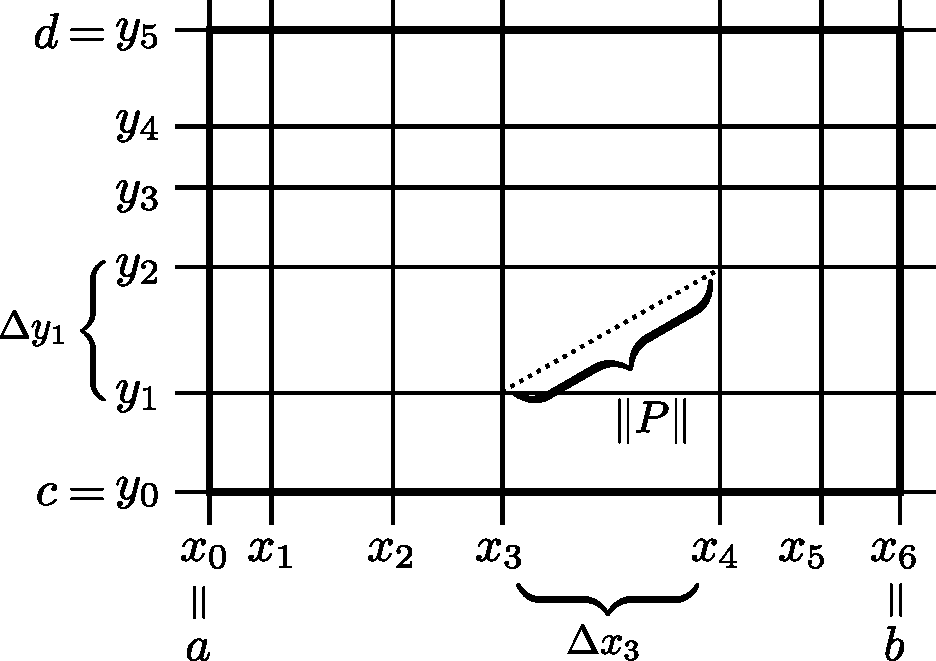
\includegraphics[width=.5\linewidth]{skipting.pdf}
            \caption*{}
\end {figure}
\end {frame}


\begin{frame}{Riemann-summa} 

\begin {block}{Skilgreining \kaflanr.\arabic{mycount}}\stepcounter{mycount}
  
 Látum $f$ vera fall skilgreint á rétthyrningi $R=[a,b]\times[c,d]$ og
 látum $P$ vera skiptingu á $R$.  Veljum úr hverjum rétthyrningi
 $[x_i,x_{i+1}]\times [y_j,y_{j+1}]$ punkt $(x_i^*, y_j^*)$.  
Skilgreinum \emph{Riemann-summuna}
$$\mathcal{R}(f,P)=\sum_{i=1}^m\sum_{j=1}^n f(x_i^*, y_j^*)\Delta x_i\Delta
  y_j.$$

   \begin {figure}[h!]
 \centering
            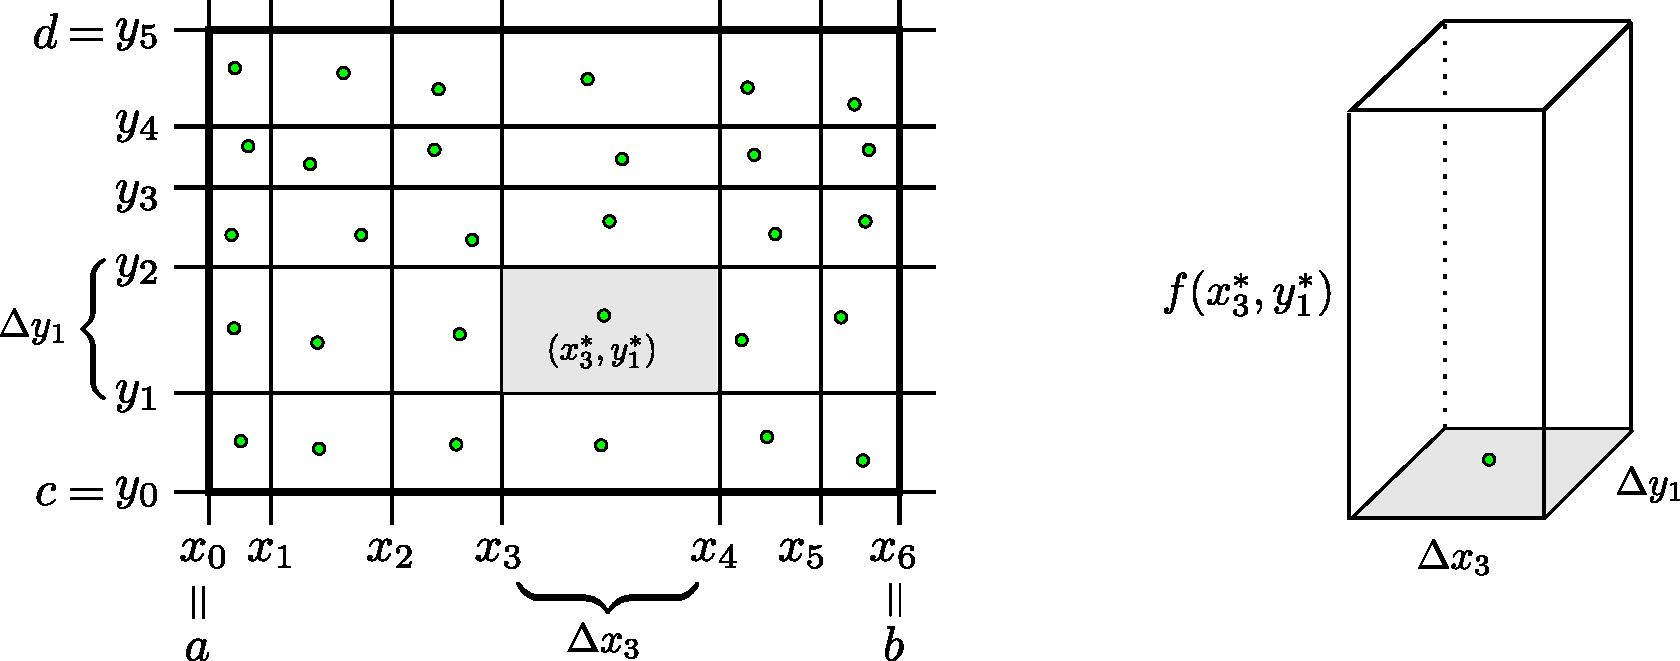
\includegraphics[width=.95\linewidth]{skipting2.pdf}
            \caption*{}
\end {figure}
\end{block}

\end{frame}

\begin {frame}
    \begin {figure}[h!]
 \centering
            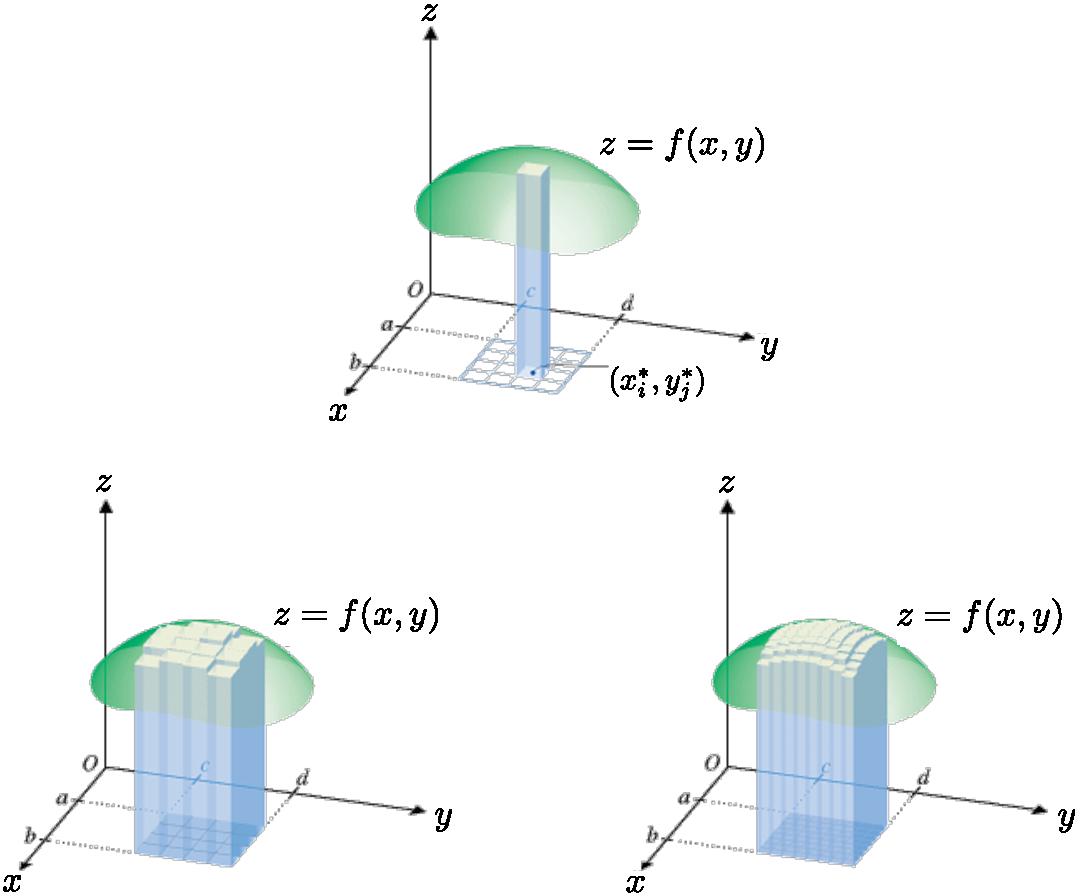
\includegraphics[width=0.9\linewidth]{double.pdf}
            \caption*{}
\end {figure}
\end {frame}


\begin{frame}{\nopagebreak Tvöfalt heildi yfir rétthyrning} 

\begin {block}{\nopagebreak Skilgreining \kaflanr.\arabic{mycount}}\stepcounter{mycount}
Sagt er að fall $f$ skilgreint á
rétthyrningi $R=[a,b]\times [c,d]$ sé {\em heildanlegt yfir} $R$ með
heildi $I$ (hér stendur $I$ fyrir tölu) ef fyrir sérhvert
$\epsilon>0$ er til tala $\delta>0$ 
þannig að $|\mathcal{R}(f,P)-I|<\epsilon$ fyrir allar skiptingar $P$ með
$\|P\|<\delta$ óháð vali á punktunum $(x_i^*, y_j^*)$.

Ritum þá 
$$\tvint_R f(x,y)dA=I.$$
\end{block}

\end{frame}



\begin{frame}{Tvöfalt heildi yfir takmarkað svæði} 

\begin {block}{Skilgreining \kaflanr.\arabic{mycount}}\stepcounter{mycount}
Látum $D$ vera takmarkað svæði í planinu.
Fall $f$ er sagt heildanlegt yfir $D$ ef til er rétthyrningur $R$ sem
inniheldur $D$ og fallið 
$$\hat{f}(x,y)=\left\{\begin{array}{rcl}
f(x,y)& & \mbox{ef }(x,y)\in D,\\
0& & \mbox{ef }(x,y)\in R\setminus D
\end{array}\right.$$
er heildanlegt yfir $R$.
\end{block}

\end{frame}


\begin{frame}{Tvöfalt heildi yfir takmarkað svæði} 

\begin {block}{Setning \kaflanr.\arabic{mycount}}\stepcounter{mycount}
Látum $f$ vera samfellt fall skilgreint á
lokuðu og takmörkuðu svæði $D$ í planinu $\R^2$.  Gerum ráð fyrir að
jaðar $D$ samanstandi af endanlega mörgum ferlum sem hafa endanlega
lengd.  Þá er fallið $f$ heildanlegt yfir $D$.
\end{block}

\end{frame}


\begin{frame}{} 

\begin {block}{Setning \kaflanr.\arabic{mycount}}\stepcounter{mycount}
Látum $D$ vera svæði í planinu og $f$ takmarkað
fall skilgreint á $D$ og heildanlegt yfir $D$.  Þá gildir:

\begin {enumerate}
 \item $\tvint_D f(x,y)\,dA=0$ ef flatarmál $D$ er 0.
 \item $\tvint_D 1\,dA=$ flatarmál $D$.
 \item Ef $f(x,y)\geq 0$ fyrir alla punkta $(x,y)$ í $D$ þá er 
$\tvint_D f(x,y)\,dA$ jafnt rúmmáli rúmskikans sem liggur milli $D$ og
grafsins $z=f(x,y)$.
\item Ef $f(x,y)\leq 0$ fyrir alla punkta $(x,y)$ í $D$ þá er 
$\tvint_D f(x,y)\,dA$ jafnt mínus rúmmáli rúmskikans sem liggur milli $D$ og
grafsins $z=f(x,y)$.
\end {enumerate}

\end{block}

\end{frame}


\begin{frame}{} 

\begin {block}{Setning \kaflanr.\arabic{mycount}}\stepcounter{mycount}
Ef $D$ er svæði í planinu og $f$ og $g$
heildanleg föll yfir $D$ þá gildir:

\begin {enumerate}
 \item  Ef $L$ og $M$ eru fastar þá er
$$\tvint_D Lf(x,y)+Mg(x,y)\,dA=L\!\tvint_D f(x,y)\,dA+M\!\tvint_D
g(x,y)\,dA.$$
\item  Ef $f(x,y)\leq g(x,y)$ þá er 
$$\tvint_D f(x,y)\,dA\leq \tvint_Dg(x,y)\,dA.$$

\item  Þríhyrningsójafna: 
\scalebox{1}{$\qquad\bigg|\tvint_D f(x,y)\,dA\bigg|\leq \tvint_D |f(x,y)|\,dA.$}

\item  Ritum $D$ sem sammengi af svæðum $D_1,\ldots, D_k$ sem skarast
ekki nema mögulega í jaðarpunktum þá er
$$\tvint_D f(x,y)\,dA=\sum_{i=1}^k\tvint_{D_i}f(x,y)\,dA.$$
\end {enumerate}

\end{block}

\end{frame}


\begin{frame}{} 

\begin {block}{Setning Fubinis \kaflanr.\arabic{mycount}}\stepcounter{mycount}

Látum $f$ vera fall sem er heildanlegt yfir rétthyrning $R=[a,b]\times
[c,d]$. Setjum
$$A(x)=\int_c^d f(x,y)\,dy\qquad\mbox{($x$ hugsað sem fasti þegar heildað)}.$$
Þá gildir að 
$$\tvint_R f(x,y)\,dA=\int_a^b A(x)\,dx=\int_a^b\!\!\int_c^d
f(x,y)\,dy\,dx.$$
Sömuleiðis gildir þegar við setjum 
$$A(y)=\int_a^b f(x,y)\,dx\qquad\mbox{($y$ hugsað sem fasti þegar heildað)} \qquad \text{að}$$
$$\tvint_R f(x,y)\,dA=\int_c^d A(y)\,dy=\int_c^d\!\!\int_a^b
f(x,y)\,dx\,dy.$$

\end{block}

\end{frame}
\begin {frame}
    \begin {figure}[h!]
 \centering
            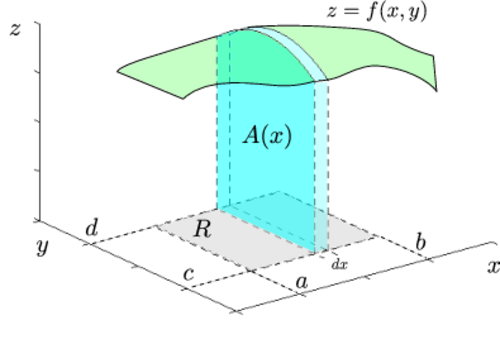
\includegraphics[width=0.6\linewidth]{ax1}
            \caption*{}
\end {figure}
\end {frame}
\end{document}